%% ------------- Portuguese version ------------
% \documentclass{sbrt}
% \usepackage[english,brazil]{babel}
% \usepackage[utf8]{inputenc}
% \newtheorem{theorem}{Teorema}
%% ---------------------------------------------

%% If writing in English, remove the lines above
%% and uncomment the lines below

%% ------------- English version ---------------
\documentclass[english]{sbrt}
\usepackage[english]{babel}
\usepackage[utf8]{inputenc}
\usepackage{cite}
\usepackage{graphicx}
\usepackage{float}
\usepackage[top=2cm,left=2cm,right=3cm,bottom=3cm]{geometry}
\usepackage{titlesec}
\newtheorem{theorem}{Theorem}
%% ---------------------------------------------

\titlespacing*{\section}
  {0pt}{18pt}{18pt}
  
\titlespacing*{\subsection}
  {0pt}{18pt}{18pt}

\begin{document}

\title{Multiplayer game (a decidir título)}

\author{Tiago da Silva Guerreiro and Lucas Costa dos Prazeres
    \thanks{Special thanks to professor Eduardo Cerqueira, ITEC, UFPA, Belém-PA, e-mail: cerqueira@ufpa.br}%
}

\maketitle

\baselineskip = 18pt


\begin{abstract}
    abstract.
\end{abstract}
\begin{keywords}
    keywords.
\end{keywords}

\section{\textbf{Introduction}}
Falar sobre o nosso projeto, nossos objetivos com ele e seus componentes

\section{\textbf{Background}}
Discorrer brevemente sobre websockets (como a interação ocorre, suas etapas, etc). É interessante ser coisas que citaremos na parte da simulação.

\section{\textbf{Game}}
The game is a simple web and multiplayer version of the classic snake game, in which a player needs to
"catch" as many fruits as possible to earn more points.

\begin{figure}[H]
  \centering
  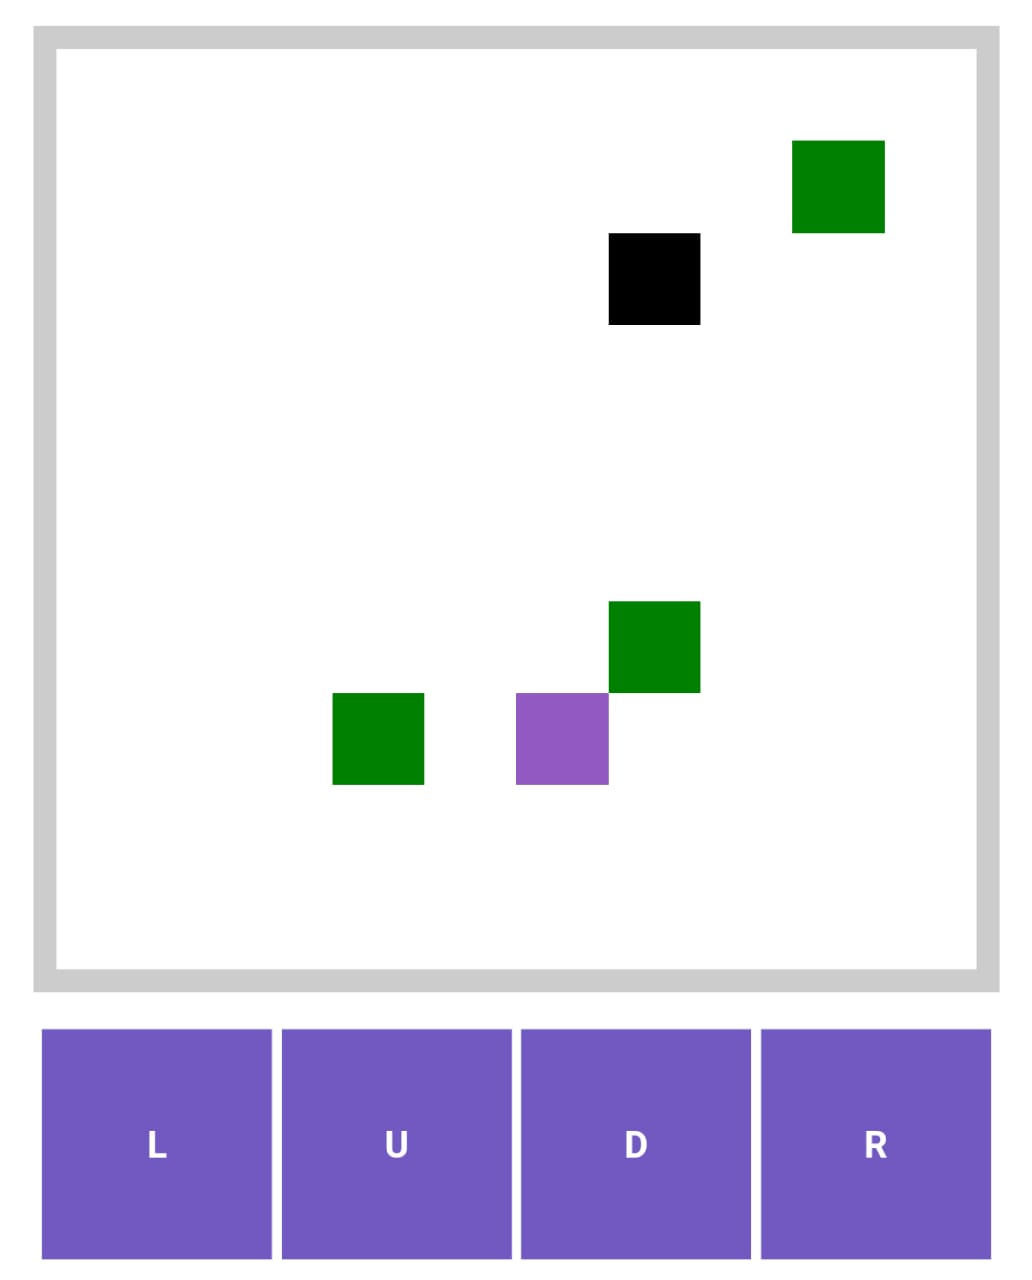
\includegraphics[width=5cm]{game-screen.jpg}
  \caption{screenshot of the game with 2 players and 3 fruits available}
\end{figure}

The project is composed by a few JavaScript files containing the main logic and also the network settings, besides an HTML with embed JavaScript with the game interface and client-side code. The platform for the server code is the NodeJS runtime, while the client code gets executed by the players browser. Its structure is simple and yet, it has a well-defined architecure, as shown below on figure [x].

\begin{figure}[H]
  \centering
  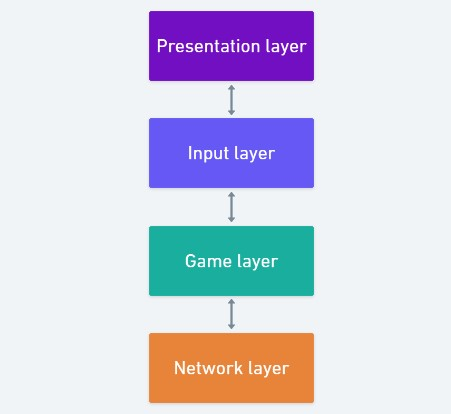
\includegraphics[width=8cm]{game-layers.jpg}
  \caption{game layers}
\end{figure}

The first layer from top to bottom is the presentation layer, which contains the HTML responsible for rendering the page and also the required definitions for the other modules to work.
The following layer is the input layer which handles the user inputs and propagate them to next layer. The third layer is the game layer which contains the bulk of the game logic and rules
applied to all its players and its algo responsible for interpreting the commands notifyed by the input listenter layer above. At this level, the game state is represented as a data structure containing
all player and fruit abstractions which are manipulated locally and propagated to the server and then to the other clients. The last layer is the network one, in which is possible to see the actual communication logic.
Now, its important to understand how the game is setup and how the hosts interact with each other.

\begin{figure}[H]
  \centering
  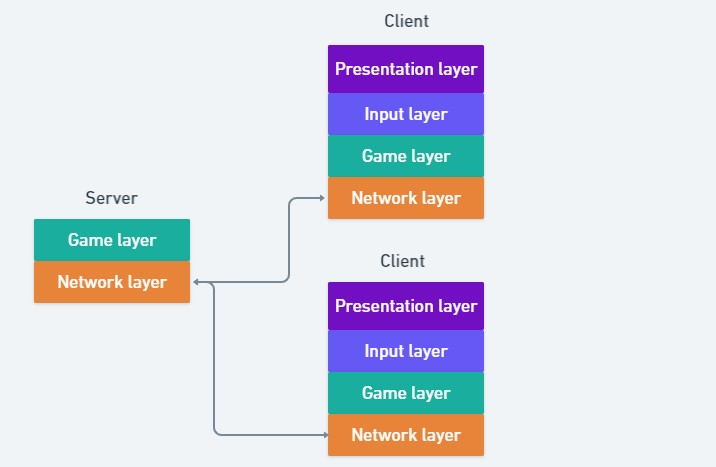
\includegraphics[width=12cm]{game-diagram.jpg}
  \caption{hosts interaction diagram}
\end{figure}

As shown in the figure above the game consists of a server and a few clients. When the server file is executed, it uses the game layer to create its own game state and the Nodejs libraries express and socketio to create a web server and a websocket server, both listening on port 3000.
Then, the client request the game page via regular HTTP request, which is reponded with the game HTML file and its javascript dependencies. After the clients receive the page, a websocket connection is started and the first message from server to the client contains the current
game state data structure, which is used by the client side to render the game screen. Meawhile, on the server side a new websocket connection is registered and an "add-player" message its propagated to all the previously connected clients and also changes the game state on the server.
Every time a player moves, leaves the page or triggers another kind of event, its own game state is updated and a notification is sent to the server, which is responsible for syncronizing all players states by notifying them too.

\section{\textbf{Simulation}}
Fazer a simulação da perda de pacotes que o professor sugeriu, ou alguma outra interessante (talvez achemos alguma na leitura dos papers).

\section{\textbf{Conclusion}}
Concluir o trabalho daquele jeito tradicional, comentando sobre os resultados.

\cite{maodv01} Pra não dar erro.

\bibliography{sbrt}
\bibliographystyle{IEEEtran}

\end{document}
